% =============================================================
% Appendix -- technical appendix after the References, as in the shared Word version.
% The former supplementary material is reduced to Table A (detail of Table 8) and the
% training curves; the LoRA-vs-DINOcow maps and the alpha / learning-curve figure were dropped.
% =============================================================
\clearpage
\section*{Appendix}
\addcontentsline{toc}{section}{Appendix}

\ifmarcas\noindent\bx{cO}{\small Optional in JDS (technical appendix). The whole Appendix can be removed.}\par\fi

\subsection*{Graphing the thresholds for BCS--DIM visualization}

\begin{marca}{cO}
To assess the herd's BCS tendency and region contribution in the 37 \mE{cows} with known DIM, target scores were tailored to the specific stage in the lactation cycle.
It is recommended that a cow has a BCS between 2.75 and 3.25 at the time she is dried off.
During the final three to four weeks before calving, known as the dry or precalving period, maintaining a BCS between 3.25 and 3.75 is considered optimal for subsequent lactation performance.
At calving, the ideal target narrows to a BCS of 3.0 to 3.5, with scores exceeding 3.75 strongly discouraged, as they increase the risk of metabolic disorders and reduced appetite.
Following calving, some loss of body condition is expected, and a BCS between 2.5 and 3.0 during the peak lactation period (0--60 DIM) is normal.
As milk production begins to decline, cows should regain condition, aiming for a BCS of 2.75 to 3.25 in mid-lactation (61--200 DIM) and 3.0 to 3.5 in late lactation (beyond 200 DIM) to ensure adequate energy reserves for the next calving cycle \citep{roche2009}.
This is represented as seen in \mR{\mbox{Figure~\ref{fig:french}}}.
\end{marca}

\begin{figure}[!htbp]
  \centering
  \bx{cO}{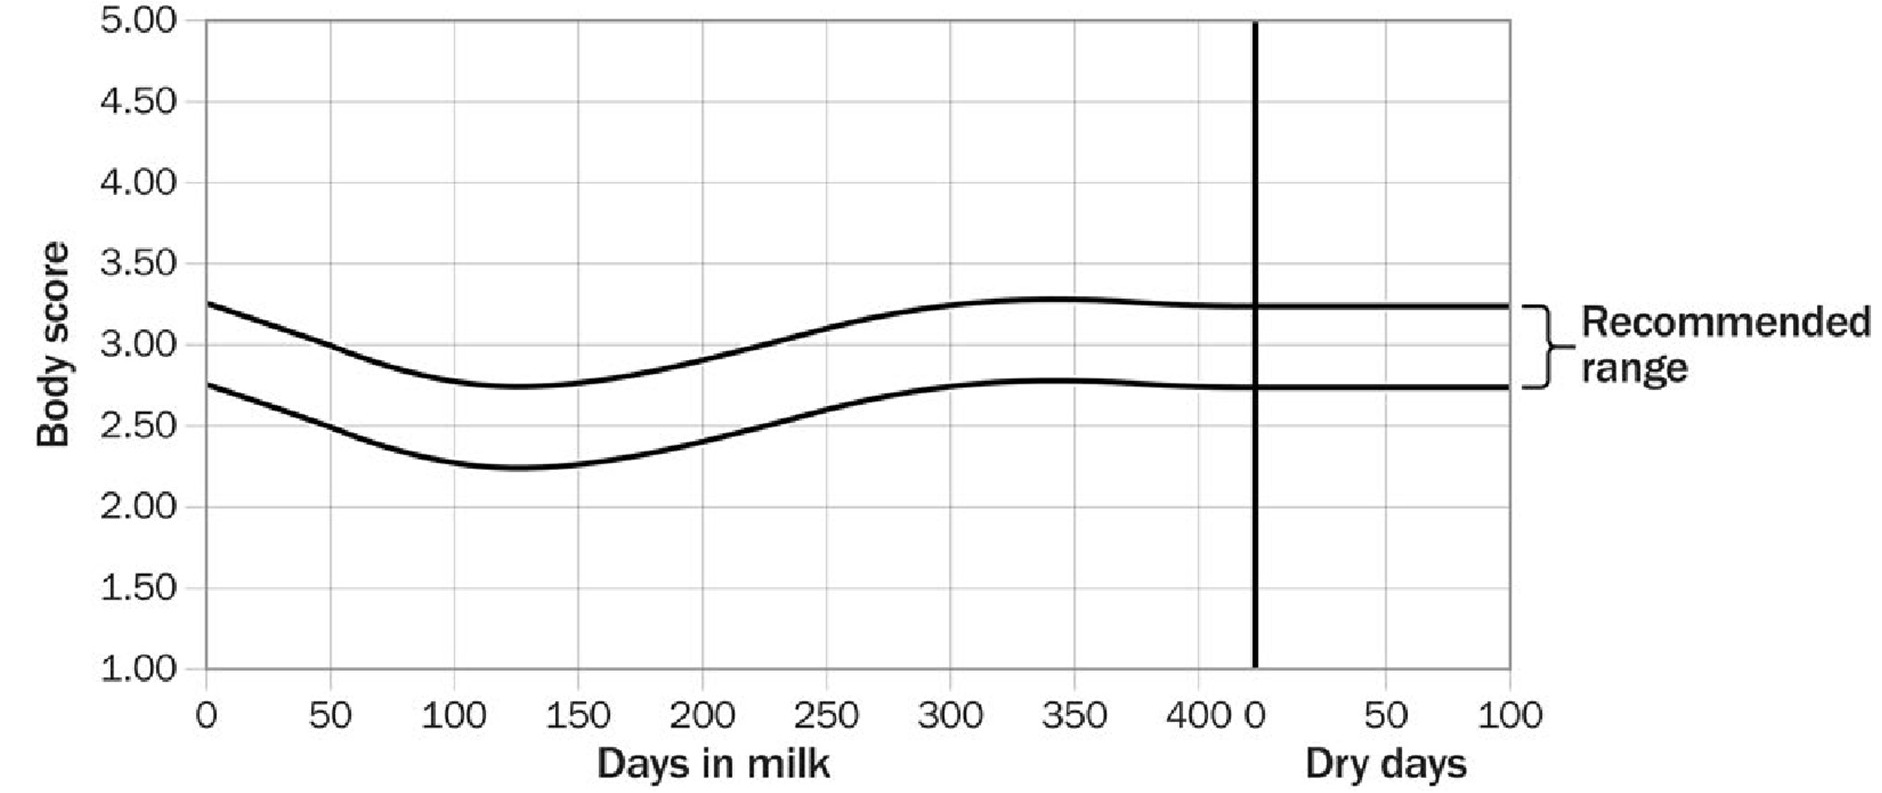
\includegraphics[width=0.8\linewidth]{../figures/word/french_bcs.jpg}}
  \caption{Dairy herd body condition score chart with lactation curve in mind \citep{french2020}.}
  \label{fig:french}
\end{figure}

\begin{marca}{cO}
The chart of \citet{french2020} gives the recommended band only as a drawing, so its center line was approximated by a fourth-degree polynomial in days in milk, fitted by least squares to nine points read from the chart every 50 days between 0 and 400 DIM,
\begin{equation}
  c(\mathrm{DIM}) = 3.00 - 0.8599\,t + 0.1946\,t^{2} + 0.0693\,t^{3} - 0.0163\,t^{4},
  \qquad t = \frac{\mathrm{DIM}}{100} ,
  \label{eq:french}
\end{equation}
where the constant was set to 3.00 so that the curve starts at the target score at calving.
Writing the polynomial in hundreds of days keeps every coefficient on the same scale as the score.
The healthy range at a given DIM is $c(\mathrm{DIM}) \pm 0.25$, rounded to the 0.25 grid of the scale, and beyond 400 DIM it is fixed at 2.75--3.25.
\end{marca}

\begin{marca}{cO}
For the figures, the reference curve was instead adapted to the targets of \citet{roche2009}, which place the lowest condition near peak lactation and a recovery towards the end of lactation,
\begin{equation}
  r(\mathrm{DIM}) = 3.50 - 0.76\,\frac{\mathrm{DIM}}{65}\, e^{\,1-\mathrm{DIM}/65} - 0.19\,\frac{\mathrm{DIM}}{305} ,
  \qquad r(\mathrm{DIM}) = r(305) \ \text{for}\ \mathrm{DIM} > 305 .
  \label{eq:roche}
\end{equation}
The second term is a loss of condition that peaks at 65 DIM, and the third a slow linear decline over a 305-day lactation.
The curve starts at 3.50 at calving, reaches its minimum of 2.70 at about 65 DIM and returns to 3.22 at 305 DIM, within 0.13 points of the anchor points used to draw \mR{\mbox{Figure~\ref{fig:semaforo}}} (3.50, 3.00, 2.75, 3.00, 3.20 and 3.25 at 0, 30, 75, 180, 270 and 305 DIM).
\end{marca}

\begin{marca}{cO}
The predicted BCS of the 37 cows with a confirmed ID in the robotic milking system was placed at the corresponding DIM, so that each prediction could be read against the reference curve \mR{\mbox{(Figure~\ref{fig:contrib}a)}}.
Each prediction was then assigned a categorical health indicator with a traffic-light scheme.
Green indicates that the cow lies within the healthy range for its DIM, yellow that it shows a moderate deviation of at most 0.25 BCS units outside that range, and red that it deviates further.
\end{marca}

\pendiente{Confirm with the authors of range.py and CurvaLactancia.py (i) why the points read from the chart were lowered by 0.07 and the constant set to 3.00 (in total Eq.~\ref{eq:french} lies 0.14 below the chart); (ii) Eq.~\ref{eq:french} reaches its minimum of 2.30 at about 155 DIM, later and lower than Eq.~\ref{eq:roche}, so the system and the figures use different targets; (iii) the origin of the coefficients of Eq.~\ref{eq:roche} (0.76, 65, 0.19), which are not in the code, and whether Figure~\ref{fig:semaforo} cites \citet{xavier2022} or \citet{roche2009}.}

\begin{figure}[!htbp]
  \centering
  \bx{cO}{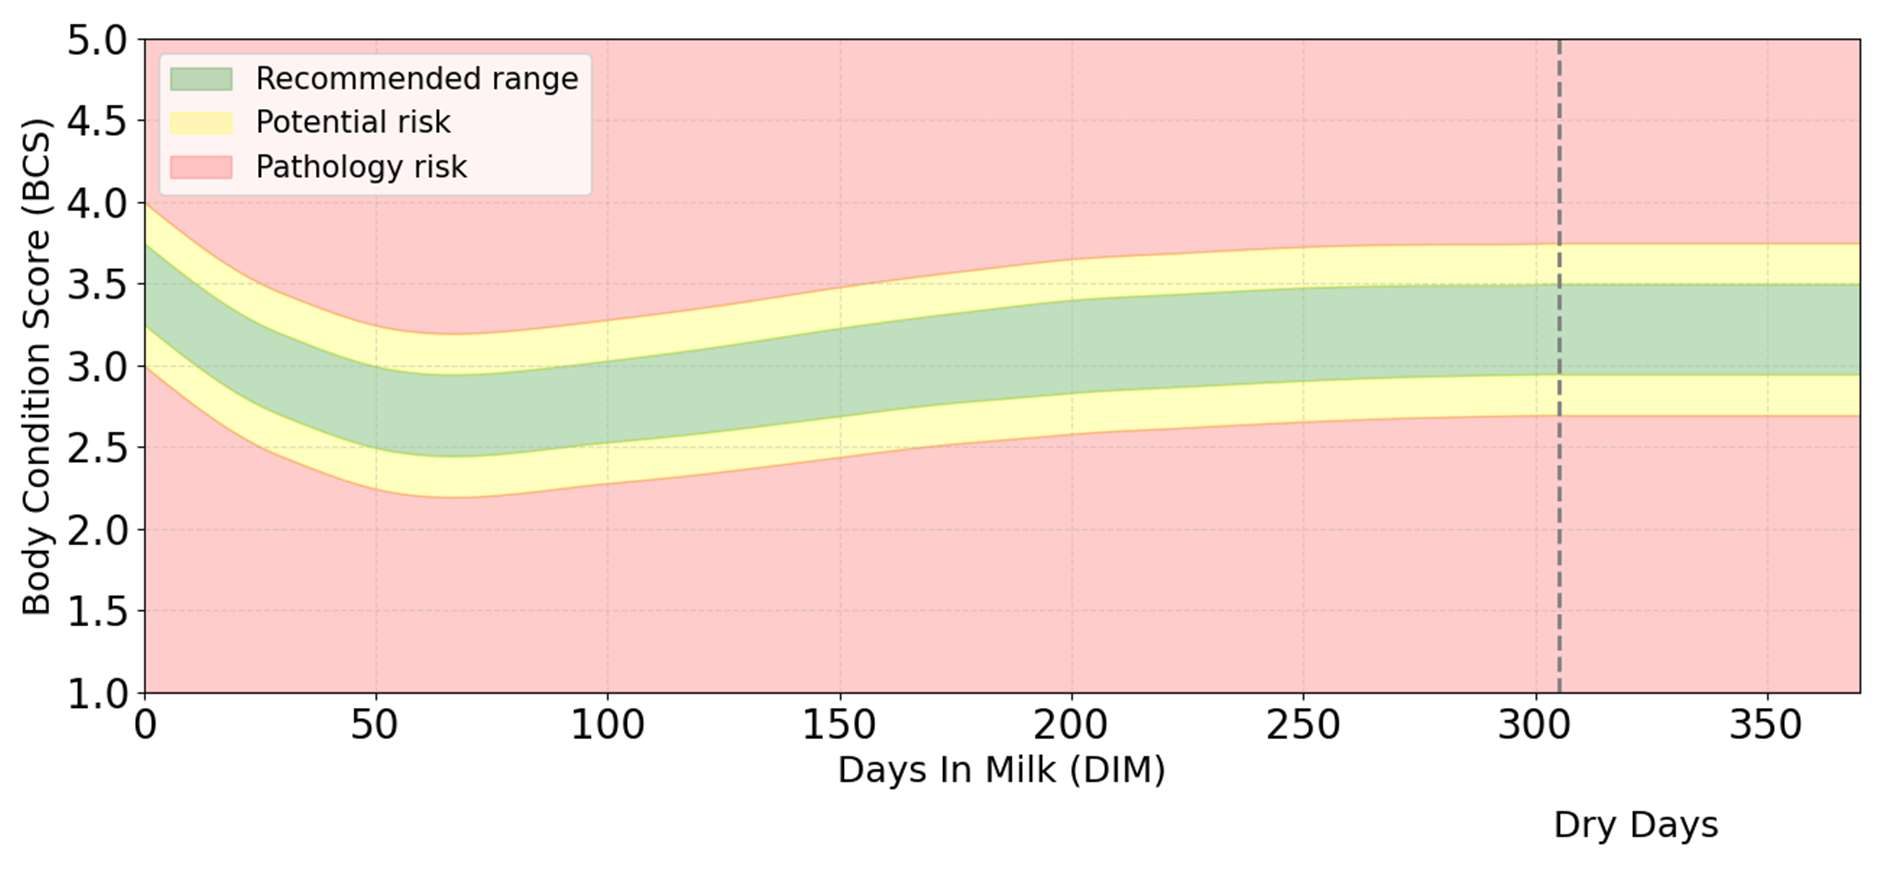
\includegraphics[width=0.8\linewidth]{../figures/word/semaforo_bcs.jpg}}
  \caption{\mE{Traffic-light zones of BCS along the lactation. The reference curve follows the shape of the body weight curve of \mbox{\citet{xavier2022}}, with anchor points adjusted to the BCS targets of \mbox{\citet{roche2009}} for early, mid and late lactation. Green marks the recommended range, yellow a deviation of at most 0.25 points outside it (potential risk) and red a larger deviation (pathology risk). The dashed line marks the end of a 305-day lactation.}}
  \label{fig:semaforo}
\end{figure}

\pendiente{Source of the 0.25 yellow margin and of the width of the green band.}

\begin{marca}{cO}
\mR{\mbox{Figure~\ref{fig:lactancia}}} was built in the same way, with anchor points joined by PCHIP interpolation.
The milk yield curve follows the lactation curve clusters that \citet{lee2020} obtained with the K-medoids algorithm, the live weight curve follows the body weight changes during lactation reported by \citet{xavier2022}, and the dry matter intake (DMI) curve follows the responses to short-term changes in supplementation reported by \mE{\mbox{\citet{souza2025}}}.
The relative timing of the three curves was checked against the diagram of \citet{martinet1999} \mR{\mbox{(Figure~\ref{fig:martinet})}}.
This diagram was preferred to the DMI equation of \mE{\mbox{\citet{nrc2021}}}, because that equation adjusts DMI for BCS and DIM rather than describing the average course of each variable.
\end{marca}

\begin{figure}[!htbp]
  \centering
  \bx{cO}{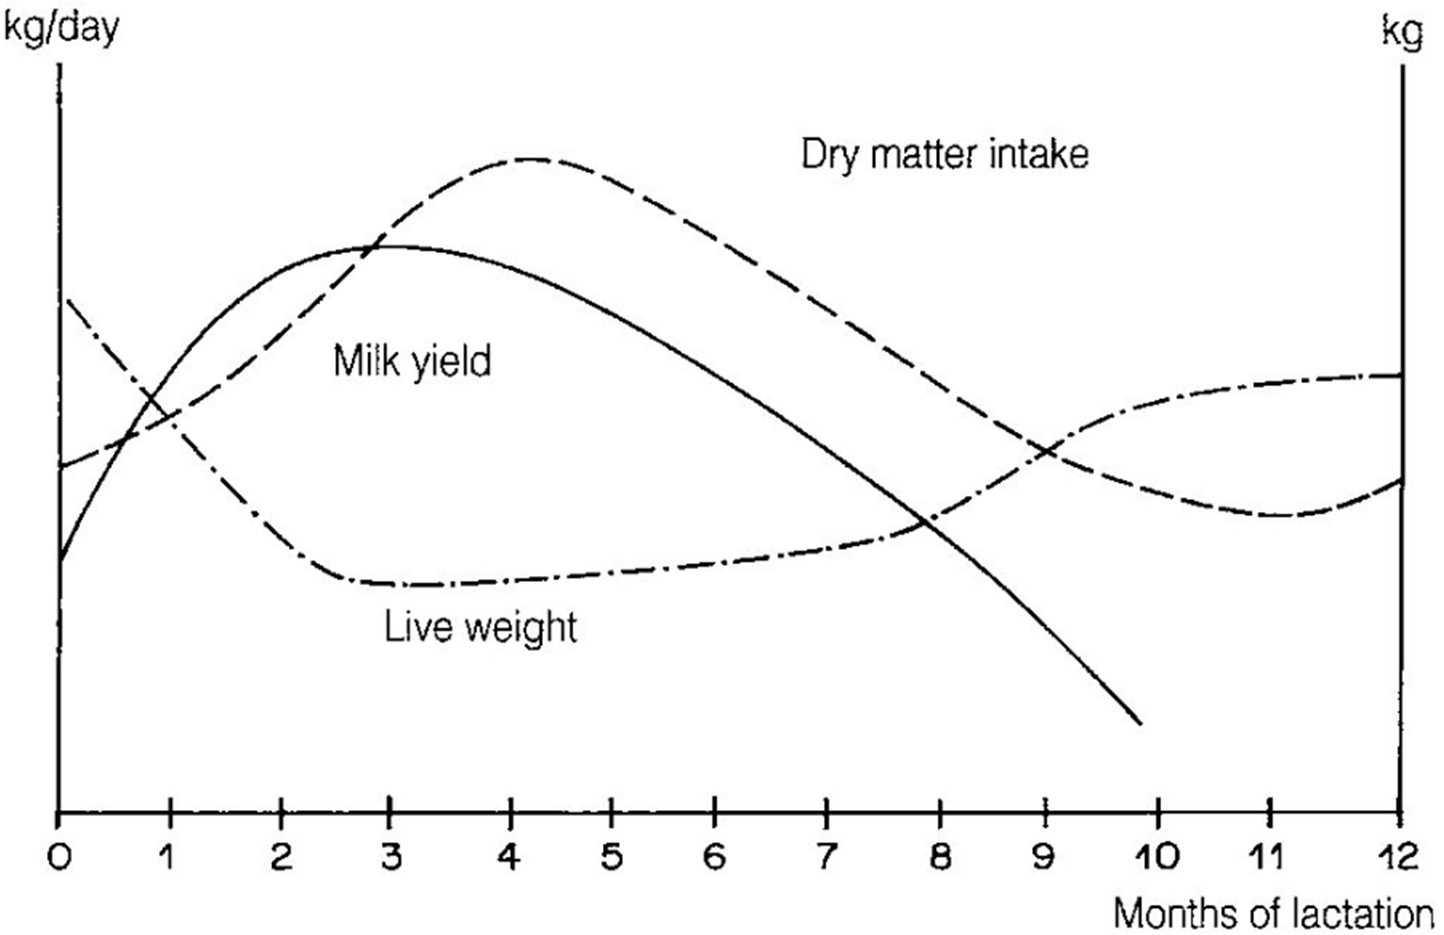
\includegraphics[width=0.7\linewidth]{../figures/word/martinet.jpg}}
  \caption{Associations among milk yield, dry matter intake and body weight during a lactation and gestation cycle \mE{(adapted from \mbox{\citealp{martinet1999}})}.}
  \label{fig:martinet}
\end{figure}

\pendiente{Confirm the name of the NASEM (2021) DMI equation (``Moore equation''?). Reproducing the diagram of Martinet et al.\ (1999) needs the publisher's permission.}

\begin{marca}{cO}
In \mR{\mbox{Figure~\ref{fig:contrib}}} the herd trend is above the reported average in BCS\mE{. This} can be explained by the fact that cows in pen 6 at CAETEC were of diverse DIM, so dietary planning became more complex without grouping animals by milk yield and lactation stage, and because some \mE{cows'} diets were not adjusted to the lowering milk yield, animals tended towards over conditioning during late lactation \citep{schroder2006}.
Additionally, lactation lengths exceeding 400 days were due to prolonged lactation periods, where even if it can result in lower milk yield \citep{jukna2024}, it is a common practice of dairy producers in hot areas of northern Mexico \citep{mellado2016}.
\end{marca}

\subsection*{Baselines, training behavior and DINOcow error}

\begin{marca}{cO}
Table~\ref{tab:detalle} extends Table~\ref{tab:summary}, with predictions averaged over the three seeds. Bias is the mean signed error for thin ($<3$) and fat ($\geq4.5$) cows.
\end{marca}

\begin{table}[!htbp]
  \centering
  \caption{Detailed comparison with the baselines on unseen cows (5 cow-level folds $\times$ 3 seeds)}
  \label{tab:detalle}
  \bx{cO}{\resizebox{\textwidth}{!}{%
  {\begin{tabular}{lcccccccc}
    \toprule
    Method & MAE $\downarrow$ & RMSE $\downarrow$ & $R^2$ $\uparrow$ & $\pm0.5$ $\uparrow$ & MAE/cow $\downarrow$ & $\Delta$ MAE/cow [95\% CI] $\downarrow$ & Bias thin $\to0$ & Bias fat $\to0$ \\
    \midrule
    \textbf{DINOcow (our model)} & \textbf{0.428} & \textbf{0.537} & \textbf{0.70} & \textbf{75\%} & \textbf{0.414} & -- & \textbf{+0.53} & \textbf{$-$0.29} \\
    DINOcow, 80\% of training cows & 0.438 & 0.544 & \textbf{0.70} & 72\% & 0.424 & +0.010 [$-$0.003, +0.024] & +0.54 & $-$0.33 \\
    DINOv3 + LoRA, regions & 0.433 & 0.539 & \textbf{0.70} & \textbf{75\%} & 0.428 & +0.014 [$-$0.018, +0.046] & +0.57 & $-$0.35 \\
    DINOv3 + LoRA & 0.437 & 0.557 & 0.68 & \textbf{75\%} & 0.434 & +0.020 [$-$0.025, +0.066] & +0.57 & $-$0.35 \\
    ResNet-50, fine-tuned & 0.656 & 0.795 & 0.35 & 58\% & 0.614 & +0.200 [+0.131, +0.270] & +1.06 & $-$0.53 \\
    EfficientNet-V2-S, fine-tuned & 0.639 & 0.759 & 0.41 & 55\% & 0.625 & +0.211 [+0.152, +0.272] & +0.98 & $-$0.60 \\
    ViT-B/16, fine-tuned & 0.660 & 0.811 & 0.32 & 53\% & 0.628 & +0.215 [+0.152, +0.282] & +0.98 & $-$0.60 \\
    ResNet-50, frozen + ridge & 0.652 & 0.805 & 0.34 & 55\% & 0.642 & +0.228 [+0.165, +0.293] & +0.86 & $-$0.68 \\
    EfficientNet-B0, fine-tuned & 0.726 & 0.880 & 0.21 & 50\% & 0.667 & +0.253 [+0.179, +0.331] & +1.22 & $-$0.65 \\
    YOLO11s-cls & 0.740 & 0.903 & 0.16 & 47\% & 0.707 & +0.293 [+0.211, +0.381] & +1.14 & $-$0.73 \\
    YOLOv8s-cls & 0.775 & 0.907 & 0.16 & 41\% & 0.713 & +0.299 [+0.220, +0.384] & +1.05 & $-$0.86 \\
    \bottomrule
  \end{tabular}}}}
\end{table}

\begin{figure}[!htbp]
  \centering
  \bx{cO}{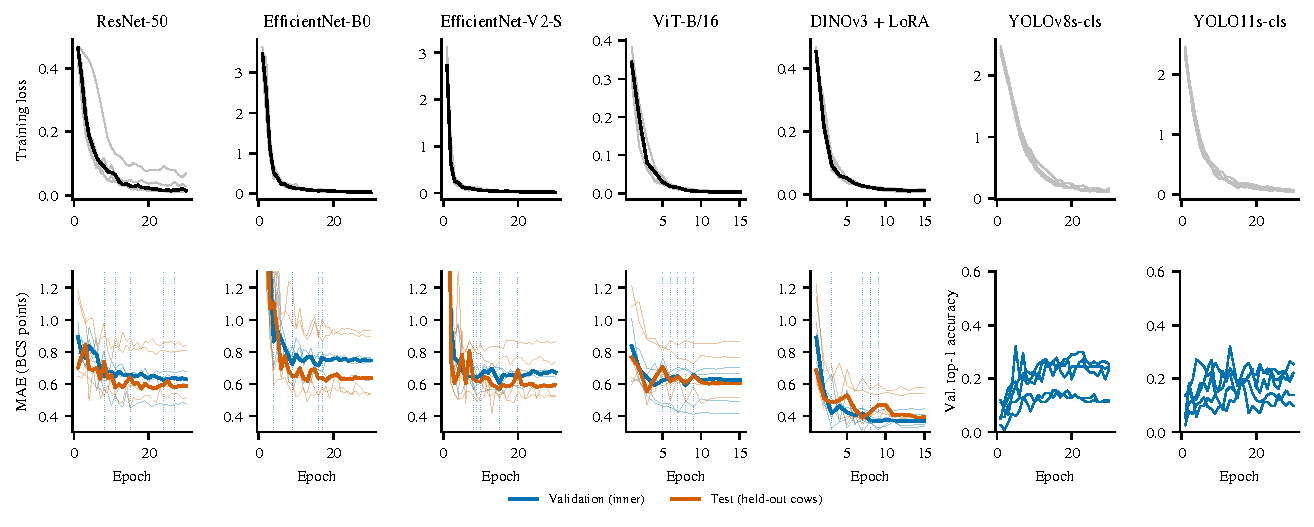
\includegraphics[width=\textwidth]{../figures/curvas_entrenamiento.pdf}}
  \caption{Training curves of the fine-tuned baselines (seed 0). Top, training loss. Bottom, validation and test error.}
  \label{fig:curvas}
\end{figure}
